\documentclass[aspectratio=169]{beamer}

%\usepackage[table]{xcolor}
\mode<presentation> {
  \usetheme{Boadilla}
%  \usetheme{Pittsburgh}
%\usefonttheme[2]{sans}

%\usepackage{lmodern}
%\usepackage[T1]{fontenc}
%\usepackage{palatino}
%\usepackage{cmbright}

\useinnertheme{rectangles}
}
%\usepackage{normalem}{ulem}
%\usepackage{colortbl, textcomp}
\setbeamercolor{normal text}{fg = black}
\setbeamercolor{structure}{fg = blue}
\definecolor{trial}{cmyk}{1,0,0, 0}
\definecolor{trial2}{cmyk}{0.00,0,1, 0}
\definecolor{darkgreen}{rgb}{0,.4, 0.1}
\definecolor{mygray}{gray}{0.8}
\definecolor{myblack}{rgb}{0, 0, 0}
\usepackage{array}
\beamertemplatesolidbackgroundcolor{white}  \setbeamercolor{alerted
text}{fg=red}

\setbeamertemplate{caption}[numbered]\newcounter{mylastframe}

\usepackage{color}
\usepackage{tikz}
\usetikzlibrary{arrows}
\usepackage{colortbl}
\usepackage{graphicx}
\usepackage{epsfig}

%\usepackage[usenames, dvipsnames]{color}
%\setbeamertemplate{caption}[numbered]\newcounter{mylastframe}c
%\newcolumntype{Y}{\columncolor[cmyk]{0, 0, 1, 0}\raggedright}
%\newcolumntype{C}{\columncolor[cmyk]{1, 0, 0, 0}\raggedright}
%\newcolumntype{G}{\columncolor[rgb]{0, 1, 0}\raggedright}
%\newcolumntype{R}{\columncolor[rgb]{1, 0, 0}\raggedright}

%\begin{beamerboxesrounded}[upper=uppercol,lower=lowercol,shadow=true]{Block}
%$A = B$.

%\usepackage[all]{xy}

\usepackage{tikz}
\usepackage{lipsum}

 \newenvironment{changemargin}[3]{%
 \begin{list}{}{%
 \setlength{\topsep}{0pt}%
 \setlength{\leftmargin}{#1}%
 \setlength{\rightmargin}{#2}%
 \setlength{\topmargin}{#3}%
 \setlength{\listparindent}{\parindent}%
 \setlength{\itemindent}{\parindent}%
 \setlength{\parsep}{\parskip}%
 }%
\item[]}{\end{list}}
\usetikzlibrary{arrows}
%\usepackage{palatino}
%\usepackage{eulervm}
\usecolortheme{lily}

\newtheorem{com}{Comment}
\newtheorem{lem} {Lemma}
\newtheorem{prop}{Proposition}
\newtheorem{thm}{Theorem}
\newtheorem{defn}{Definition}
\newtheorem{cor}{Corollary}
\newtheorem{obs}{Observation}
 \numberwithin{equation}{section}


\title[PLSC 43401]
{Mathematical Foundations of Political Methodology Lecture 5}

\author{Robert Gulotty}
\institute[University of Chicago]{Department of Political Science \\  University of Chicago}
\vspace{0.3in}
\date{August 28th, 2020}

\setbeamertemplate{navigation symbols}{}

\begin{document}




\begin{frame}
\titlepage
\end{frame}


\begin{frame}

\begin{itemize}
\item Last time we learned about the Mean Value Theorem.
\item We will briefly return to that topic before turning to techniques for finding maxima and minima.
\item How much can we infer about the value of a function at a point $x$ given the curvature at a point $x_0$?
\end{itemize}

\end{frame}



\begin{frame}{Linear Approximation.}

\begin{itemize}
\item We want to know $f(b)$, we know $f(a)$, $f'(a)$ 

\item With the slope and the distance between a and b we can calculate the position of $f(b)$:
$$f(b)\approx f(a)+(b-a)f'(a)$$
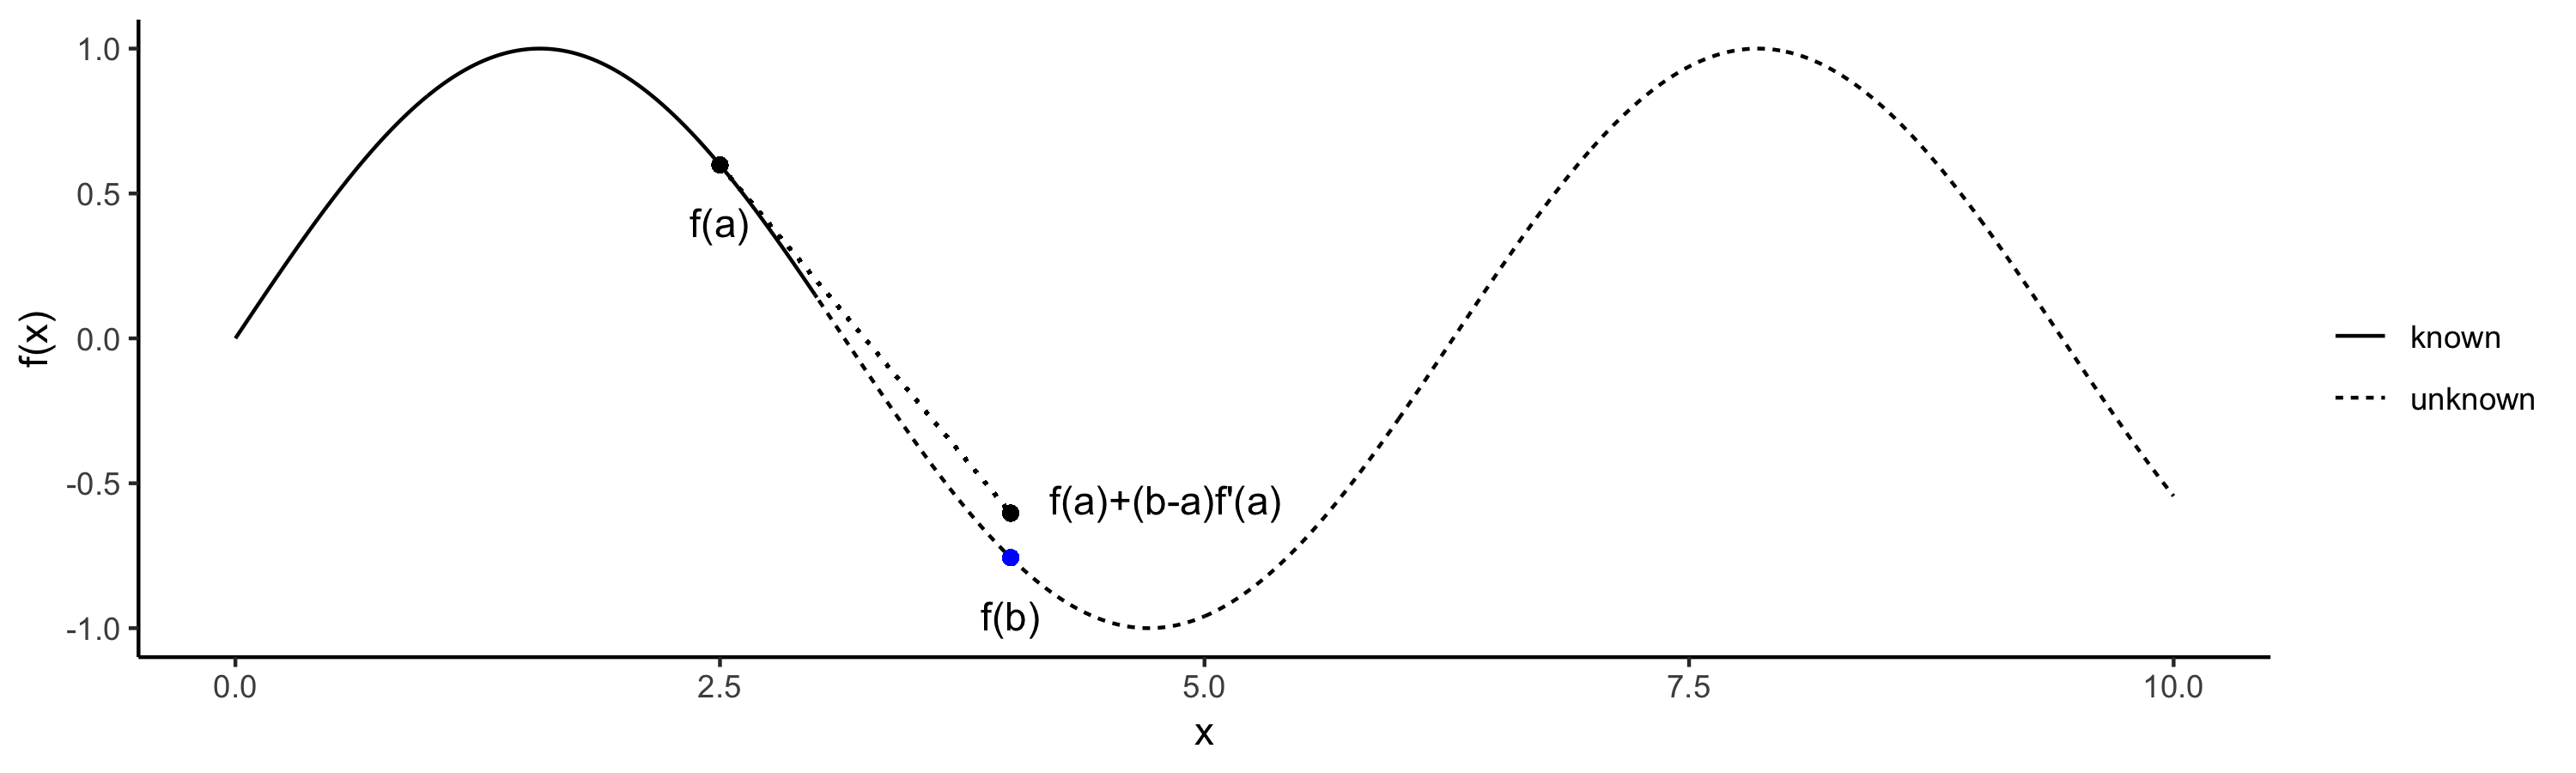
\includegraphics[width=4.5 in]{approx.png}\pause
\item Can we do better? 
\end{itemize}

\end{frame}


\begin{frame}{Preliminary Result: Second Mean Value Theorem (pg 189).}

\begin{thm} If $f$ is a twice-differentiable function and $a$ and $b$ are real numbers such that $a<b$, there exists $d$ such that $a<d<b$ and 
$$f(b)=f(a)+(b-a)f'(a)+\frac{1}{2}(b-a)^2f''(d)$$
\end{thm}

\end{frame}


\begin{frame}{Applying the Second MVT}

$$f(b)=f(a)+(b-a)f'(a)+\frac{1}{2}(b-a)^2f''(d)$$\pause
Set $b=a+h$, $d=a+th$ for some $0<t<1$:

$$f(a+h)=f(a)+(h)f'(a)+\frac{1}{2}(h)^2f''(a+th)$$\pause
If $|h|$ isn't too big:
$$f(a+h)\approx f(a)+(h)f'(a)+\frac{1}{2}(h)^2f''(a)$$\pause
Replace $h=x-a$, 
$$\tilde{f}(x)=f(a)+(x-a)f'(a)+\frac{1}{2}(x-a)^2f''(a)$$

$\tilde{f}(x)$ is called the quadratic approximation of $f(x)$



\end{frame}



\begin{frame}{Moving to Taylor's Theorem}
\begin{itemize}
\item The best approximation uses higher order derivatives.\pause
\item If a function has arbitrary many higher derivatives, it is called smooth.  \pause
\item We use these higher derivatives to approximate a function to arbitrary precision.
\end{itemize} 
\end{frame}

\begin{frame}{Taylor's Theorem}
If $f$ is a smooth function and n is a positive integer:
{\scriptsize
$$f(a+h)=f(a)+hf'(a)+\frac{h^2}{2}f''(a)+\frac{h^3}{3!}f'''(a)+...+\frac{h^{n-1}}{(n-1)!}f^{(n-1)}(a)+\frac{h^{n}}{(n)!}f^{(n)}(a+th)$$\pause
}
The (n-1)th order Taylor approximation sets the nth term to 0:
$$f(a+h)\approx f(a)+hf'(a)+\frac{h^2}{2!}f''(a)+\frac{h^3}{3!}f'''(a)+...+\frac{h^{n-1}}{(n-1)!}f^{(n-1)}(a)+0$$
 

\end{frame}

\begin{frame}{Taylor's Series Expansion}

In general, the Taylor's Approximations take advantage of Taylor's Series:
$$f(a+h)=f(a)+hf'(a)+\frac{h^2}{2}f''(a)+\frac{h^3}{3!}f'''(a)+...$$
is a convergent series.\pause
\begin{itemize}
\item The Taylor Expansion plays a starring role in the Central Limit Theorem, the main result of the second half of this class.\pause
\item It is also used to characterize the exponential function $e$.\pause
$$e^x=f(x)=f'(x)=f''(x)...$$\pause
\item[] Note that $e^0=1$.  Set $a=0$\pause

$$e^{0+h}=1+h+\frac{h^2}{2!}+\frac{h^3}{3!}...$$

\end{itemize}

\end{frame}

\begin{frame}{Binomial Series}



\end{frame}


\begin{frame}{Binomial Series}
\begin{itemize}
\item We saw that $e^x$ can be expanded into something that multiplies $x^0,\ x^1,\ x^2 \ldots$, 
\item the book shows the same is true for $ln(1+x)$. 
\item An important example of these power series is:
$$f(x)=(1+x)^c$$
\item This formula gives rise to the \emph{Binomial Series}.
\end{itemize}
\end{frame}

\begin{frame}{Binomial Series $f(x)=(1+x)^c$}
\begin{align*}
f(x)&=(1+x)^c\\
f'(x)&=c(1+x)^{c-1}\\
f''(x)&=c(c-1)(1+x)^{c-2}\\
f''(x)&=c(c-1)(c-2)(1+x)^{c-3}
\ldots
\end{align*}
\end{frame}


\begin{frame}{Binomial Series $f(x)=(1+x)^c$}
Consider f(0):
\begin{align*}
f(0)&=(1)^c\\
f'(0)&=c(1)^{c-1}\\
f''(0)&=c(c-1)(1)^{c-2}\\
f''(0)&=c(c-1)(c-2)(1)^{c-3}
\ldots
\end{align*}
\end{frame}


\begin{frame}{Binomial Series $f(x)=(1+x)^c$}
Consider f(0):
\begin{align*}
f(0)&=1\\
f'(0)&=c\\
f''(0)&=c(c-1)\\
f''(0)&=c(c-1)(c-2)
\ldots
\end{align*}
\end{frame}


\begin{frame}{Binomial Series $f(x)=(1+x)^c$}
Call $a_1=c$, $a_2=\frac{c-1}{2}$, $a_3=\frac{c-2}{3}\ldots$ $a_k=\frac{c-(k-1)}{k}$\pause
\begin{align*}
f(0)&=1\\
f'(0)&=c=a_1\\
f''(0)&=c(c-1)=2*1*a_1a_2\\
f''(0)&=c(c-1)(c-2)=3*2*1*a_1a_2a_3
\ldots
\end{align*}

\end{frame}

\begin{frame}{Binomial Series $f(x)=(1+x)^c$}
Call $a_1=c$, $a_2=\frac{c-1}{2}$, $a_3=\frac{c-2}{3}\ldots$ $a_k=\frac{c-(k-1)}{k}$\pause
\begin{align*}
f(0)&=1\\
f'(0)&=c=1! a_1\\
f''(0)&=c(c-1)=2! a_1a_2\\
f''(0)&=c(c-1)(c-2)=3!a_1a_2a_3
\ldots
\end{align*}
\end{frame}




\begin{frame}{Binomial Series $f(x)=(1+x)^c$}
Call $a_1=c$, $a_2=\frac{c-1}{2}$, $a_3=\frac{c-2}{3}\ldots$ $a_k=\frac{c-(k-1)}{k}$
Applying the Taylor series:
$$f(0+x)= f(0)+xf'(0)+\frac{x^2}{2!}f''(0)+ \frac{x^3}{3!}f'''(0)\ldots$$\pause
We get:
$$(1+x)^c=1+a_1x+\frac{2*a_1a_2}{2!}x^2+\frac{3!a_1a_2a_3}{3!} x^3 \ldots$$\pause
$$(1+x)^c=1+a_1x+a_1a_2x^2+a_1a_2a_3 x^3 \ldots$$
\end{frame}

\begin{frame}{Binomial Series $f(x)=(1+x)^c$}
Call $a_1=c$, $a_2=\frac{c-1}{2}$, $a_3=\frac{c-2}{3}\ldots$ $a_k=\frac{c-(k-1)}{k}$\\
Suppose $c$ is a positive integer $m$:\pause
$$a_{m}=\frac{m-(m-1)}{m}=1$$\pause
$$a_{m+1}=\frac{c-(m+1-1)}{m+1}$$\pause
$$a_{m+1}=\frac{m-m}{m+1}=0$$

$$(1+x)^c=1+a_1x+a_1a_2x^2+a_1a_2a_3 x^3 \ldots$$
$$(1+x)^m=1+mx+\frac{m(m-1)}{2!}x^2+\frac{m(m-1)(m-3)}{3!} x^3 +\ldots +1* x^m +0$$
\end{frame}

\begin{frame}{Binomial Series $f(x)=(1+x)^c$}
$$(1+x)^m=1+mx+\frac{m(m-1)}{2!}x^2+\frac{m(m-1)(m-3)}{3!} x^3 +\ldots +1* x^m $$
$$(1+x)^m={m \choose 0}x^0+{m \choose 1}x+{m \choose 2}x^2+{m \choose 3} x^3 +\ldots +{m \choose r} x^r+ \ldots + {m \choose m}x^m$$

where:
$${m \choose r} =\frac{m(m-1)(m-2)\ldots (m+1-r)}{r!}=\frac{m!}{r!(m-r)!}$$
\end{frame}



\begin{frame}{Binomial Series Example: $f(x)=(1+x)^5$}
$$(1+x)^5={5 \choose 0}x^0+{5 \choose 1}x+{5 \choose 2}x^2+{5 \choose 3} x^3 +{5 \choose 4} x^4+{5 \choose 5}x^5$$
$$(1+x)^5=1+5x+10 x^2+10 x^3 +5 x^4+x^5$$
\end{frame}

\begin{frame}{Pascal's Triangle}
\begin{tabular}{>{$n=}l<{$\hspace{12pt}}*{13}{c}}
0 &&&&&&& ${ 0 \choose 0}$ &&&&&&\\
1 &&&&&& ${ 1 \choose 0}$ && ${ 1 \choose 1}$&&&&&\\
2 &&&&& ${ 2 \choose 0}$ && ${ 2 \choose 1}$ && ${ 2 \choose 2}$ &&&&\\
3 &&&& ${ 3 \choose 0}$ && ${ 3 \choose 1}$ && ${ 3 \choose 2}$ && ${ 3 \choose 3}$ &&&\\
4 &&& ${ 4 \choose 0}$ && ${ 4 \choose 1}$ && ${ 4 \choose 2}$ &&${ 4 \choose 3}$ && ${ 4 \choose 4}$ &&\\
5 && ${ 5 \choose 0}$ && ${ 5 \choose 1}$ && ${ 5 \choose 2}$ && ${ 5 \choose 3}$ && ${ 5 \choose 4}$ && ${ 5 \choose 5}$ &\\
6 & ${6 \choose 0}$ && ${6 \choose 1}$ && ${6 \choose 2}$ && ${6 \choose 3}$ && ${6 \choose 4}$ && ${6 \choose 5}$ && ${ 6 \choose 6}$
\end{tabular}
\end{frame}


\begin{frame}{Pascal's Triangle}
\begin{tabular}{>{$n=}l<{$\hspace{12pt}}*{13}{c}}
0 &&&&&&&1&&&&&&\\
1 &&&&&&1&&1&&&&&\\
2 &&&&&1&&2&&1&&&&\\
3 &&&&1&&3&&3&&1&&&\\
4 &&&1&&4&&6&&4&&1&&\\
5 &&1&&5&&10&&10&&5&&1&\\
6 &1&&6&&15&&20&&15&&6&&1
\end{tabular}
\end{frame}

\begin{frame}

\begin{itemize}
\item \textcolor{myblack}{Monotone and Inverse Functions}
\item \textcolor{myblack}{Second Derivative Test}
\item \textcolor{myblack}{Global Maxima}
\item \textcolor{myblack}{Convex and Concave Functions}
\end{itemize}

\end{frame}



\begin{frame}

\begin{itemize}
\item \textcolor{myblack}{Monotone and Inverse Functions}
\item \textcolor{mygray}{Second Derivative Test}
\item \textcolor{mygray}{Global Maxima}
\item \textcolor{mygray}{Convex and Concave Functions}
\end{itemize}

\end{frame}



\begin{frame}
\frametitle{Monotone Functions}

\begin{defn}
Monotonic functions: functions that are either \textit{strictly increasing} or \textit{strictly decreasing}
\end{defn} \pause

\begin{itemize}
\item Strictly increasing: If $x_2>x_1$ then $f(x_2)>f(x_1)$
\item Strictly decreasing: If $x_2>x_1$ then $f(x_2)<f(x_1)$ \pause
\item If $f^\prime(x)>0$ for all $x$, then $f$ is strictly increasing; \\however this is stronger than we need for a function to be strictly increasing (e.g. $f(x)=x^3$)
\item If $f^\prime(x)\geq 0$ for all $x$ and $f^\prime(x)=0$ for only a finite number of $x$, then $f$ is strictly increasing (with strictly decreasing proved similarly)
\end{itemize}

\end{frame}



\begin{frame}
\frametitle{Inverse Functions}

\begin{defn}
Let $f(x)$ be monotonic.  Then for any $y$, $f(x)=y$ has at most one solution. If the solution is written $x=g(y)$, then $g$ is the \textit{inverse function} of $f$, or $$f(g(y))=y \hbox{ and }g(f(x))=x$$
\end{defn} \pause

\ \\Example 1:  Let $f(x)=x^3$; what is the inverse function of $f$? \pause

\ \\Example 2: Let $f(x)=x^{-1}+5$; what is the inverse function of $f$? \pause

\ \\The inverse function is a reflection of the function about the $45^\circ$ line; what's the inverse of the function $\{(1, 2),(2, 3), (3, 4)\}$?

\end{frame}



\begin{frame}
\frametitle{The inverse function rule}

\ \\If $f$ is monotonic with inverse function $g$, and for a given $x$, $f$ is differentiable and $f^\prime(x)\not=0$, then $$g^\prime(y) = \frac{1}{f^\prime(x)}$$ \pause


\ \\This gives us another technique for differentiating things; we could calculate $f^\prime$ directly, or we could calculate $\frac{1}{g^\prime}$

\end{frame}




\begin{frame}
\frametitle{Critical Points}

\ \\If $f^\prime(x)=0$ then $x$ is called a \textit{critical point}

\begin{itemize}
\item Maximum
\item Minimum
\item Inflection point
\end{itemize}

\begin{center}
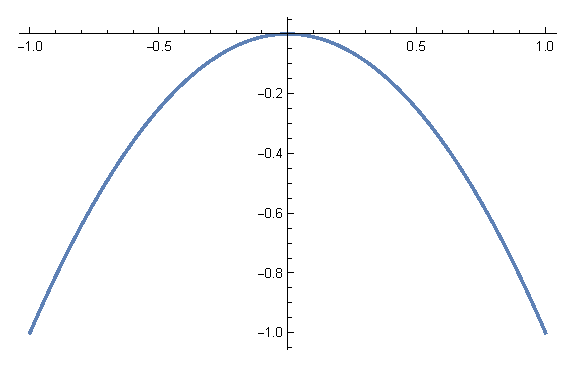
\epsfig{file=max.eps, scale=.32} 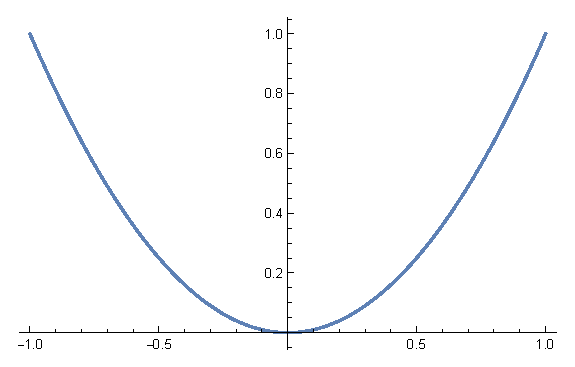
\epsfig{file=min.eps, scale=.32} 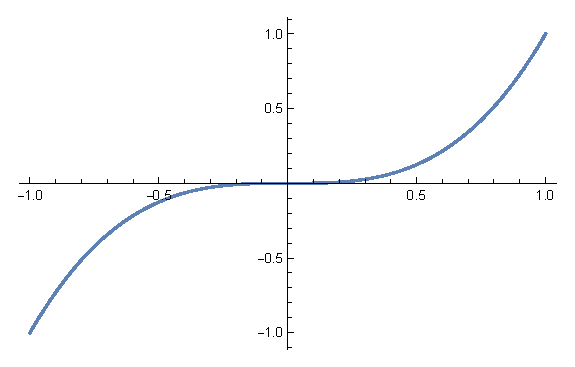
\epsfig{file=inflect.eps, scale=.32}
\end{center}

\end{frame}



\begin{frame}
\frametitle{Critical Points}

One of the main things we use calculus for is to identify and classify critical points \pause

\begin{enumerate}
\item Find $f^\prime(x)$ \pause
\item Find the set of $x$ such that $f^\prime(x)=0$ \pause
\item Intuitively, if $f^\prime(x)$ changes from negative to positive around $x$, then $x$ is a minimum; if it changes from positive to negative then $x$ is a maximum; if it does neither then it's a point of inflection \pause
\item Always remember that without more knowledge of $f$, all we know is that $x$ is a \textit{local} maximum or minimum (or an inflection point); we can't assume that it maximizes or minimizes our function globally
\end{enumerate}

\end{frame}



\begin{frame}

\begin{itemize}
\item \textcolor{mygray}{Monotone and Inverse Functions}
\item \textcolor{myblack}{Second Derivative Test}
\item \textcolor{mygray}{Global Maxima}
\item \textcolor{mygray}{Convex and Concave Functions}
\end{itemize}

\end{frame}



\begin{frame}
\frametitle{Second Derivative Test}

Recall that if $f^\prime$ is itself differentiable, then $f$ is \textit{twice differentiable}, and $f^{\prime\prime} = \frac{d^2y}{dx^2}$ is the \textit{second derivative} \pause

\begin{itemize}
\item Suppose that $f^{\prime\prime}(x)$ is positive at some point $x$ \pause
\item This means that the \textit{slope of the slope} of $f$ is increasing at $x$ \pause
\item This means that either:

\begin{itemize}

\item If $f$ is increasing then it's increasing at an increasingly faster rate at $x$ \pause
\item If $f$ is decreasing then it's decreasing at an increasingly slower rate at $x$ \pause
\item If $f$ is flat then it's increasing as $x$ increases \pause

\end{itemize}
\item In all of these cases, $f$ lies above its tangent
\end{itemize}

\end{frame}



\begin{frame}
\frametitle{Second Derivative Test}

\begin{itemize}

\item[A] If $f$ is increasing then it's increasing at an increasingly faster rate at $x$ \pause
\item[B] If $f$ is decreasing then it's decreasing at an increasingly slower rate at $x$ \pause
\item[C] If $f$ is flat then it's increasing as $x$ increases

\end{itemize}

\vspace{.2in}
\begin{center}

\epsfig{file=convex.eps, scale=.75}
\end{center}

\end{frame}



\begin{frame}
\frametitle{Second Derivative Test}

\begin{itemize}
\item For any critical point, $x^*$, calculate $f^{\prime\prime}(x^*)$ \pause

\begin{itemize}
\item If $f^{\prime\prime}(x^*)>0$ then $x^*$ is a local minimum \pause
\item If $f^{\prime\prime}(x^*)<0$ then $x^*$ is a local maximum \pause

\item If $f^{\prime\prime}(x^*)=0$ then we don't know what $x^*$ is; we have to examine our function around $x^*$ \pause

\end{itemize}

\item $f^\prime(x)=0$ is our first-order condition; conditions on $f^{\prime\prime}$ are our second-order conditions \pause

\end{itemize}

\ \\Find and classify the critical points of $x^3-3x$, and then use this information to plot out the function

\end{frame}



\begin{frame}

\begin{itemize}
\item \textcolor{mygray}{Monotone and Inverse Functions}

\item \textcolor{mygray}{Second Derivative Test}
\item \textcolor{myblack}{Global Maxima}
\item \textcolor{mygray}{Convex and Concave Functions}
\end{itemize}

\end{frame}



\begin{frame}
\frametitle{Global Maxima}

\ \\If $f(x^*)\geq f(x)$ for all $x\in \mathbb{R}$ then $x^*$ is a global maximum \pause

\begin{itemize}
\item Global maxima survive ``strictly increasing functions''.\pause
\item[-] Suppose that $g(x)=H(f(x))$ where $H$ is a \textit{strictly increasing function}.  Then if $f$ has a global maximum at $x^*$, $g(x)$ also has a global maximum at $x^*$ \pause
\begin{itemize}
\item One useful strictly increasing function is the natural log:
\item If $x^*$ globally maximizes log$(f(x))$ then $x^*$ also maximizes $f(x)$ \pause
\end{itemize}

\item If $x^*$ is the global max of $f(x)$ then $x^*$ is the global minimum of $-f(x)$ \pause
\end{itemize}

\end{frame}



\begin{frame}
\frametitle{Existence of global maximum and minimum}

\begin{theorem}
The extreme value theorem:  any continuous function on a closed and bounded interval attains a global maximum and minimum
\end{theorem} \pause

\end{frame}

\begin{frame}
\frametitle{Boundary Conditions \& Asymptotes}

\begin{itemize}
\item Often functions have max and min at the boundaries or at asymptotes:
\item[] $y={\frac{1}{x}}$ ($x>0$) has a $x$ and $y$ asymptotes equal to the axes \pause
\item An important strategy is to trace out functions.
\item[] Trace out: $y=x-{\frac{1}{x}}$ %has asymptotes equal to the y axis and the line y=x
\end{itemize}

\end{frame}

\begin{frame}

\begin{itemize}
\item \textcolor{mygray}{Monotone and Inverse Functions}

\item \textcolor{mygray}{Second Derivative Test}
\item \textcolor{mygray}{Global Maxima}
\item \textcolor{myblack}{Convex and Concave Functions}
\end{itemize}

\end{frame}



\begin{frame}
\frametitle{Convexity and Concavity}
 
\begin{defn}
A set is \textit{convex} if the line segment connecting any two points in the set is entirely contained within the set
\end{defn}

\begin{center}
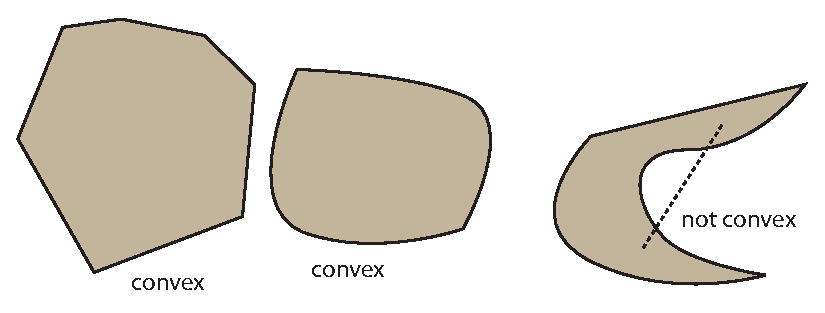
\epsfig{file=convexSet.eps, scale=.65}
\end{center}

\end{frame}



\begin{frame}
\frametitle{Convex Function}

\begin{defn}
$f$ is a convex function if and only if for all real numbers $A, B$ and all $0\leq \alpha \leq 1$, 
$$\alpha f(A)+(1-\alpha)f(B)\geq f(\alpha A+(1-\alpha)B)$$
\end{defn}

\begin{center}
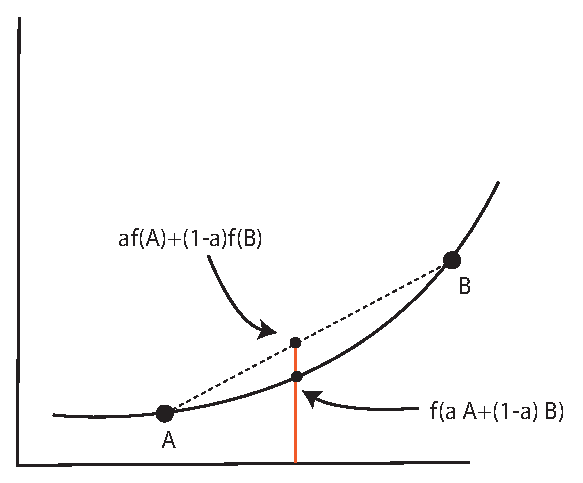
\epsfig{file=convexFunction.eps, scale=.65}
\end{center}

\end{frame}



\begin{frame}
\frametitle{Properties of Convex Functions}

Convex functions need not be differentiable (e.g. $y=|x|$). \pause

\begin{itemize}
\item If $f$ is twice differentiable, then $f$ is convex if and only if $f^{\prime\prime}\geq 0$ for all $x$ \pause

\item If $f$ is differentiable and convex then
\begin{itemize}
\item There is either no global minimum, one global minimum, or an interval of global minima \pause
\item There are no local minima that are not global minima \pause
\item If $f^\prime(x^*)=0$ then $x^*$ is a global minimum \pause
\end{itemize}
\end{itemize}

\end{frame}



\begin{frame}
\frametitle{Concave Function}

\begin{defn}
$f$ is \textit{concave} if and only if $-f$ is convex: the set of all points on or below $f$ is convex
\end{defn} \pause
\begin{itemize}
\item Concave functions are typical choices for utility functions.
\end{itemize}
\end{frame}


\begin{frame}
\frametitle{Properties of Concave Function}
\begin{itemize}
\item If $f$ is twice differentiable then $f$ is concave if and only if $f^{\prime\prime}\leq 0$ for all $x$. \pause

\item If $f$ is concave and $f^\prime(x^*)=0$ then $x^*$ is a global maximum.\pause
\item To remember, con\textbf{cave} looks like the entrance to a cave.
\end{itemize}
\end{frame}





\begin{frame}
\frametitle{Find Maxima/Minima: A Summary}

\begin{itemize}

\item Compute $f^{'}(x)$ and find all $x$ such that $f^{'}(x) = 0$; \pause

\item Conduct second derivative test, compute $f^{''}(x)$ for all $x$ such that $f^{'}(x) = 0$; \pause

\begin{itemize}
\item $f^{''}(x) > 0$, then, it's a local minimum; \pause
\item $f^{''}(x) < 0$, then, it's a local maximum; \pause
\item $f^{''}(x) = 0$, then, undecided. \pause
\end{itemize}

\item Finally, check boundary points, and determine global maxima or minima.

\end{itemize}

\end{frame}



\begin{frame}
\frametitle{Example 1: $f(x) = -x^2$,  $x \in [-3, 3] $}

	1) Critical Value:

	\begin{eqnarray}
	f^{'}(x) & = & - 2 x \nonumber \\
	0 & = & - 2 x^{*} \nonumber \\
	x^{*} & = & 0 \nonumber 
	\end{eqnarray} \pause

	2) Second Derivative: 

	\begin{eqnarray}
	f^{'}(x) & = & - 2x \nonumber \\
	f^{''}(x)  & = & - 2 \nonumber 
	\end{eqnarray}
	$f^{''}(x)< 0$, local maximum


\end{frame}

\begin{frame}
\frametitle{Example 1: $f(x) = -x^2$,  $x \in [-3, 3] $}

	3) Check end points
	\begin{eqnarray}
	f(0) & = & - 0 ^2 = 0 \nonumber \\
	f(-3) & = & - (-3)^2 = -9 \nonumber \\
	f(3) & = & - (3)^2 = -9 \nonumber 
	\end{eqnarray}

\end{frame}


\begin{frame}
\frametitle{Example 2: $f(x) = x^3$, $x \in [-3, 3] $ }

1) Critical Values: 
\begin{eqnarray}
f^{'}(x) & = & 3x^2 \nonumber \\
0 & = & 3 (x^{*})^{2} \nonumber \\
x^{*} & = & 0 \nonumber 
\end{eqnarray} \pause

2) Second Derivative: 

\begin{eqnarray}
f^{''}(x) & = & 6 x \nonumber \\
f^{''}(0) & = &  0 \nonumber 
\end{eqnarray}
\alert{No information}

\end{frame}



\begin{frame}
\frametitle{Example 2: $f(x) = x^3$, $x \in [-3, 3] $}


3) Check End Points: 

\begin{eqnarray}
f(0) & = & 0^3  = 0 \nonumber \\
f(-3) & = & -3^3 = -27 \nonumber \\
f(3) & = & 3^3 = 27 \nonumber 
\end{eqnarray}

Neither maximum nor minimum, \alert{saddle point} 

\end{frame}



\begin{frame}
\frametitle{Example 3: Spatial Model}
A large literature in Congress supposes legislators and policies can be situated in \alert{policy space} \pause \\

Suppose legislator $i$ and policies $x, i \in \mathbb{R}$. \pause  \\
Define legislator $i$'s utility as, $U:\mathbb{R} \rightarrow \mathbb{R}$, \pause 
\begin{eqnarray}
U_{i} (x) & = & - (x - \mu)^{2}  \nonumber \\ \pause 
U_{i}(x) & = & - x^2 +  2 x \mu  - \mu^2 \nonumber \pause 
\end{eqnarray}
What is $i$'s optimal policy over the range $x \in [\mu- 2, \mu + 2]$? \pause 
\begin{eqnarray}
U_{i}^{'} (x) & = & -2 (x - \mu) \nonumber \\ \pause 
0 & = & -2x^{*} + 2 \mu \nonumber \\ \pause 
x^{*} & = & \mu \nonumber \pause 
\end{eqnarray}

\alert{Second Derivative Test} \pause 
\begin{eqnarray}
U^{''}_{i}(x)  & = & -2 <0  \nonumber \pause 
\end{eqnarray}

We call $\alert{\mu}$ legislator $i$'s \alert{ideal point} 

\end{frame} 

\begin{frame}
\frametitle{Example 3: Spatial Model}

\begin{eqnarray}
U_{i}(\mu) & = & - (\mu - \mu)^2 = 0 \nonumber \\
U_{i}(\mu - 2) & = & - (\mu - 2 - \mu)^2 = -4 \nonumber \\
U_{i} (\mu + 2) & = & - (\mu + 2 - \mu)^2 = -4 \nonumber 
\end{eqnarray}

\alert{Maximize utility at $\mu$}

\end{frame}



\end{document}
